% Nama Kelompok : 
% Kelas : D4 TI 1A
% Anggota : 
% 1. Harun   	1174027
% 2. Fahmi   	1174021
% 3. Kukuh		1174016
% 4. Izzah		1174013
% 5. Rizal		1174014
% 6. Lawinner	1174030




Suatu artikel menyebutkan \cite{dale2001spacer}
Artikel tentang Bilangan Oktal.
\Section{Penjelasan Singkat}
Oktal adalah sebuah sistem bilangan berbasis delapan. Sistem bilangan ini terdiri dari 0,1,2,3,4,5,6,7 dan bilangan ini biasanya dikonversi dari biner yang berkelompok setiap 3 bit. Sistem ini mempersingkat tulisannya, agar menjadi tidak terlalu panjang. Cara baca sistem ini dari ujung paling kanan (LSB kepanjangan dari Least Significant Bit).

	\ref{Posisibilanganoktal}
	\begin{figures}[ht]
	\centerline{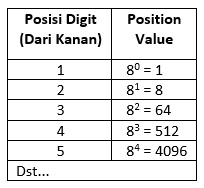
\includegraphics[width=1\textwidth]{figures/Posisibilanganoktal.JPG}}
	\caption{Perhitungan dari kanan}
	\label{Posisibilanganoktal}
	\end{figures}

Contoh contoh bilangan Oktal,
Misalnya : 
Biner Oktal
000 000 00
000 001 01
000 010 02
000 011 03
Misalnya bilangan oktal 3 adalah hasil dari pengelompokkan dari 000 011, perhitungan secara manual dapat dibuktikan dengan cara seperti berikut ini :
(1 x 21 )+(1 x 20 ) = (1×2)+(1×1) = 3

\section{Cara menghitung}
Dengan menggunakan software ms excel kita dapat melakukan konversi bilangan oktal ke bilangan heksadesimal, bilangan desimal atau pun bilangan biner.
 	\subsection{penjumlahan pada Oktal}
 ada beberapa ketentuan yang perlu kalian ketehui dalam penjumlahan bilangan oktal.dimana semua ketentuan akan digunakan pada pengurangan dan perkalian.kalau kalian belum paham betul tentang penjumlahan,saya sarankan jangan mempelajari pada tahap pengurangan dan perkalian.karena walaupun terlihat susah,namun sebenarnya sangat mudah.kunci utamanya yang perlu kalian pahami dan mempelajari ini adalah teliti,semangat da pantang menyerah.
 Hal hal yang harus paling penting harus diketahui antara lain sebagai berikut  :
1. Setiap masing - masing basis harus ditambahkan secara desimal.
2. Setelah itu , kalian harus  mengubah dari hasil desimal ke oktal.
3. Setelah diubah  , kalian harus menulis hasil dari penjumlahan digit paling kanan ke hasil bilangan oktal.
4. lalu hasil penjumlahan yang dilakukan pada tiap basis terdiri dari 2 digit , bilangan binernya nol dan 1 maka digit paling kiri merupakan  penjumlahan kolom selanjutnya.
Kemudian apabila aku menjelaskannya secara rinci , berdasarkan empat ketentuan itu , kira - kira akan seperti ini 
Soal: tambahkan bilangan 9, 6 dan 2.
Ketentuan pertama:
Tambahkan masing-masing basis secara desimal
9 + 6 + 2 = 17
Ketentuan kedua:
Ubah dari hasil desimal ke oktal.
9(8) + 7(8) + 2(8) = 17(8)
Konversikan kebilangan oktal:
17 mod 8 = 2 sisa 1
=21
Demikian cara penjumlahan berdasarkan keempat ketentuan tersebut.
Dalam hal ini bilangan oktal memiliki patokan, Yaitu sebagai berikut.

	\ref{tabelpertambahanbilanganoktal}
	\begin{figures}[ht]
	\centerline{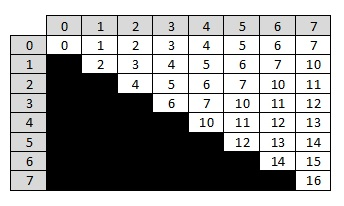
\includegraphics[width=1\textwidth]{figures/tabelpertambahanbilanganoktal.JPG}}
	\caption{Patokan Bilangan}
	\label{tabelpertambahanbilanganoktal}
	\end{figures}

Mungkin ada kalian yang bertanya: Kenapa dari 7 langsung menuju ke angka 10?
Bilangan oktal adalah bilangan yang terdiri dari 0 sampai 7 dimana nilai maksimal adalah 7. Jika lebih dari 7 maka itu  adalah pembawa dan sisanya akan kita jumlahkan pada kolom selanjutnya
1 + 6 = 7. —– > tidak lebih dari 7. Maka tetap.
1 + 7 = 8. —– > carry of 1 dan sisa 0, maka hasilnya adalah 10 (8 mod 8= hasil 1 sisa 0)
2 + 7 = 11. — > carry of 1 dan sisa 1, maka hasilnya adalah 11 (9 mod 8= hasil 1 sisa 1)
Dan seterusnya…

Ada tips yang penting Anda ketahui dan sesuatu yang harus dilaksanakan , saya menyarankan agar kalian berlatih sendiri dengan cara membuat soal dan menjawabnya sendiri . Apabila Anda sering berlatih , maka besar harapan peluang Anda akan sangat mudah untuk memahami dan akan mudah untuk menemukan jawaban-jawaban dari soal yang sangat rumit sekalipun .

	\Subsection{Pengurangan Pada Bilangan Oktal}
Sekarang kita dapat mempelajari pengurangan di bilangan oktal. Saya tidak perlu mendeskripsikan dengan jelas karena kalian pasti sudah paham dengan penjelasan sebelum nya dimana patokannya pada tabel.
Contoh:
154 – 127 = 25
Coba kalian hitung dengan kalkulator bakul beras! Apa perhitungan saya terlihat berbeda?
Lalu bagaimana dengan perhitungan oktal yang seperti ini:

154
127
____-
 
140 + (8 + 4)                        140 + 12
120 +        7                           120 +   7
__________-                    _______-
                                                20+5
                                                =25

Demikianlah contoh dari perhitungan pengurangan pada bilangan oktal . Hal ini menyebabkan kita tidak akan bergantung sepenuhnya pada kalkulator bakul beras . Mungkin seluruh Windows pasti menyediakan fitur calculator untuk para programmer . Tapi ada baiknya kita atau kalian sendiri untuk berusaha menghitungnya sendiri. Mengapa ? Karena kita akan dilatih untuk lebih teliti dalam memecahkan suatu masalah yang rumit. 
127
____-
 
140 + (8 + 4)                        140 + 12
120 +    7                           120 +   7
__________-                    _______-
                                                20+5
                                                =25

Itulah salah satu contoh dari perhitungan pengurangan bilangan oktal. Sehingga kita tidak perlu sepenuhnya bergantung terus dengan kalkulator bakul beras. Walaupun pada Windows disediakan fitur calculator untuk programmer, tapi ada baiknya kalian menghitung dengan usaha kalian sendiri. Kenapa? Agar kalian lebih teliti dalam memecahkan suatu masalah yang cukup rumit.
 
Kemudian kita akan melakukan perhitungan dengan atau tanpa digit.  
1.	Tanpa terjadi peminjaman digit.
457 – 231 = 226. Tidak percaya?? Coba hitung pake kalkulator bakul beras, calculator programmer atau kalian hitung sendiri secara manual dengan kertas dan pulpen layaknya seorang professor. Pasti hasilnya sama.
2.	Dengan peminjaman digit.
324 – 162 = 142
Apabila dijelaskan dalam pemecahan jawaban akan tampak seperti berikut:
                                200                                         200
324                           104                                          104
162-                       1  62 –                                    1   62
_____                   _____                                   _____
    2                              42                                       1   42
Mungkin kalian heran kenapa bisa ada angka 200. Jangan lupa kita berpatok pada tabel penjumlahan.
	
	\Subsection{Perkalian pada bilangan Oktal}
Penerapannya hampir sama pada penjumlahan,namun yang tak sama adalah saat yang kita gunakan adalah untuk perkalian. Setelah anda mengalikan seluruh bilangan pada kolom secara decimal, selanjunya anda menggunakan penjumlahan oktal untuk menuliskan hasilnya.
Contohnya 16 * 24:
16
24*
____
                70
             16
            _______+
            250
Apabila dideskripsikan, 6*4 = 24, kemudian dimodule 8 (24 mod 8 = 3 sisa 0). Kemudian 4 * 1 = 4 ditambah carry of 3 dari hasil penjumlahan sebelumnya (4 + 3 = 7)
Perhatikan Tabel.
0	1	2	3	4	5	6	7
0	0	0	0	0	0	0	0	0
1	1	2	3	4	5	6	7
2	4	6	10	12	14	16
3	11	14	17	22	25
4	20	24	30	34
5	31	36	43
6	44	52
7	61
cant Bit).

	\Subsection{Pembagian pada bilangan Oktal}
Pembagian bilangan oktal dapat dilakukan dengan cara yang sama, seperti pembagian bilangan desimal.
Berikut contoh soalnya :
	
5738 :  68 = . . . 8	
	 
	   77R18
	   __
	68/5738
	   52		\-\-\>6 x 7 =42
	   ____-	42 mod 8
	    53
	    52		\-\-\> \= 5 sisa 2 52
	   ____-
	   	 1
5738 : 68 = 77 R18

Untuk Angak 6 x 7 itu dari pembagi dan hasil,Kemudian jika hasilnya ada sisa,Si R itu jadi sisanya.

\Section{Fungsi Bilangan Oktal}

sebenarnya fungsi bilangan oktal itu tidak jauh beda dari fungsinya bilangan biner dan heksadesimal, yaitu sebagai kode komputasi yang untuk digunakan komputer, tetapi juga biasanya bilangan oktal dipakai sebagai pengganti heksadesimal dalam menjalankannya.

Oh ya, penasaran kenapa sih yang kita pakai dalam kehidupan sehari-hari itu desimal? karena desimal itu basis 10, menggunakan angka 0 sampai dengan 9, dan jari kita sebagai manusia yang normal ada 10, jadi itu lebih cenderung  mudah menggunakan basis 10.

Kemudian  untuk memperjelas fungsi sebelumnya, ada beberapa keuntungan dalam memakai bilangan oktal dalam komputasi dibandingkan dengan heksadesimal . Keuntungannya adalah kemudahan sistem karena tidak memerlukan simbol ekstra dan karena heksadesimal butuh simbol tambahan A-F dikarenakan basis 16 ). Selain itu , bilangan oktal juga digunakan dalam penampilan digital ( digital displays ).